\clearpage
\section{Automatyzacja i centralizacja wersjonowania projektu (JC)}
\label{ch:versioning}

Niniejsza część pracy traktuje o systemie wersjonowania stosowanym w projekcie GGSS. Zaprezentowane zostały: sposób nadawania wersji stosowany w projekcie przed rozpoczęciem prac, wymagania postawione przed przygotowanym przez autorów systemem oraz sposób jego implementacji.

\subsection{Wprowadzenie do problematyki}
Wersjonowanie oprogramowania jest to proces, którego celem jest przypisanie utworzonemu wydaniu produktu unikatowego identyfikatora, dzięki czemu w dowolnym momencie możliwy jest powrót do oznaczonej w ten sposób wersji systemu. Jest to szczególnie przydatne, gdy do środowiska produkcyjnego trafia wadliwa wersja aplikacji - możliwe jest wtedy przywrócenie odpowiedniego, testowanego wcześniej wydania. Wersjonowanie aplikacji pozwala ponadto na śledzenie zmian oraz usprawnień wprowadzanych w poszczególnych aktualizacjach. Użytkownicy są w stanie, sprawdzając dokumentację wprowadzonych zmian, określić, czy wykorzystywana przez nich wersja aplikacji posiada wszystkie wymagane funkcjonalności. Ponadto znajdywanie głównej przyczyny późno wykrytego błędu staje się znacznie prostsze, dzięki możliwości porównywania wadliwej wersji produktu z informacjami dotyczącymi wcześniejszych, działających poprawnie wydań.

W pierwotnej wersji projektu GGSS wersjonowaniu poddawany był jedynie pakiet RPM z sterownikami oraz zależnościami zewnętrznymi. Wersja składała się z czterech komponentów, czyli \lstinline{<MAJOR>.<MINOR>.<PATCH>-<RELEASE>}. Komponent wersji, który był modyfikowany przy wprowadzaniu zmian był wybierany uznaniowo. Ponadto nadawanie wersji nie było wtedy procesem automatycznym - polegało na manualnym modyfikowaniu wartości w jednym z plików \lstinline{.cmake}. Stosując takie rozwiązanie, próba wersjonowania wielu komponentów projektu wymagałaby wielokrotnego powtarzania tych samych czynności.

\subsection{Motywacja do wprowadzenia zmian}
Pierwszym czynnikiem, z powodu którego zdecydowano się na wprowadzenie zmian w systemie wersjonowania była jego nieporęczność. Każda zmiana i wydanie nowej wersji aplikacji wymagały od dewelopera, aby pamiętał, że należy jeszcze dodatkowo zmienić wersję w plikach \lstinline{.cmake}. Był to kolejny krok, który programista musiał wykonać w celu przeprowadzenia poprawnego procesu rozwoju oprogramowania, a co za tym idzie potencjalnie kolejne miejsce na pomyłkę. 

Dodatkowo niepoprawnie przeprowadzona zmiana wersji (np. na niższą) powodowała problemy z procesem instalacji nowego wydania oprogramowania w środowisku docelowym. Ze względu na to, że na systemy działające przy detektorze ATLAS nałożone są duże wymagania i ograniczenia, to proces instalacji nowych wersji aplikacji jest monitorowany przez administratorów systemowych. Pomyłki w zmianie wersji oprogramowania uniemożliwiały ich zainstalowanie ze względu na błędy w działaniu menadżera pakietów oraz sprzeciw administratorów w stosunku do instalacji niepoprawnie wersjonowanych aplikacji.

Kolejnym czynnikiem, który spowodował wprowadzenie zmian w systemie wersjonowania był wymóg postawiony autorom, aby wszystkie aplikacje GGSS publikowane w danym momencie miały nadaną dokładnie tą samą wersję. Dzięki zastosowaniu takiego podejścia możliwe jest bardzo szybkie zidentyfikowanie kombinacji komponentów systemu GGSS, które są ze sobą kompatybilne.

Ze względu na te czynniki postanowiono przygotować zautomatyzowany, scentralizowany system wersjonowania oparty o dostępną infrastrukturę, czyli: skrypty budujące napisane w języku Python, pliki \lstinline{.cmake}, portal GitLab i automatyzację w oparciu o GitLab CI/CD.

\subsection{Zmiany w skryptach budujących projekt}
W celu zapewnienia automatycznego, scentralizowanego wersjonowania należało wykonać zmiany w kilku warstwach projektu GGSS. W pierwszej kolejności zmodyfikowano główny skrypt do budowania (\lstinline{build.py}) znajdujący się w repozytorium \emph{ggss-all}. Została dodana do niego obsługa argumentu wejściowego \lstinline{--version} tak, aby można było definiować wersję zarówno manualnie (w trakcie uruchamiania wyżej wymienionego skryptu), jak i poprzez automatyzację zdefiniowaną w ramach GitLab CI/CD. W przypadku braku podania wersji, za pomocą której mają zostać oznaczone budowane pliki, postanowiono ustawiać ją tak, by możliwie łatwe było odróżnienie wydania produkcyjnego od deweloperskiego. W takim przypadku wersja przygotowywana przez skrypt wygląda następująco: \lstinline{dev-YYYY-MM-DD_HH-MM-SS}. Pozwala to na określenie, że pliki zostały zbudowane poza oficjalnym systemem automatyzującym cały proces, a ponadto taka konwencja umożliwia poznanie dokładnego momentu uruchomienia skryptu budującego. Oprócz rozszerzenia argumentów wejściowych, dostosowania wymagał również sposób obsługi plików \lstinline{.cmake} w wyżej wymienionym skrypcie. 

\subsection{Zmiany w systemie opartym o narzędzie CMake}
W przypadku plików \lstinline{.cmake} zastosowano podobne podejście, jak w przypadku pliku \lstinline{build.py}, tzn. dodano argument wejściowy w postaci parametru \lstinline{VERSION}. Pozwala to na odebranie wartości wersji od skryptów zewnętrznych, jak i manualne wpisanej przez użytkownika. W przypadku nieustawienia wartości wyżej wymienionego parametru stosowana jest wartość domyślna: \lstinline{no-version}. Listing \ref{lst:cmake_version_arg} przedstawia przykładowe zastosowanie tego systemu w przypadku repozytorium \emph{ggss-driver}.

\begin{lstlisting}[
    language=CMake,
    caption={Zastosowanie parametru \lstinline{VERSION} w repozytorium \emph{ggss-driver}.},
    label={lst:cmake_version_arg},
    frame=single
]
if(NOT VERSION)
    set(VERSION "no-version")
endif()

message(STATUS "ggss-driver version: ${VERSION}")

#parameter initialization
set(CPACK_PACKAGE_NAME "ggss-driver-cc7")
set(CPACK_PACKAGE_VERSION ${VERSION})
\end{lstlisting}


\subsection{Zastosowanie \emph{semantic-versioning} oraz zmiany w automatyzacji}
Do tej pory w projekcie GGSS wersja zmieniania była według uznania dewelopera, który wprowadzał tą informację w plikach \lstinline{.cmake} odpowiedzialnych za budowanie danego komponentu systemu. W celu ustandaryzowania tego procesu zdecydowano się na stosowanie zasad \emph{semantic-versioning} \cite{semver}, wedle których wersja powinna składać się z trzech komponentów:
\begin{itemize}
    \item \textbf{MAJOR} - komponent ten jest zmieniany, gdy wprowadzane są zmiany w interfejsie programistycznym aplikacji, przez co nie jest zachowywana kompatybilność z wcześniejszymi wydaniami, na przykład: dodatkowy, wymagany argument bez wartości domyślnej
    \item \textbf{MINOR} - komponent ten jest zmieniany, gdy w aplikacji wprowadzane są zmiany niepowodujące problemów z kompatybilnością, na przykład: dodanie nowej funkcjonalności, które nie wpływa na oferowane dotąd możliwości
    \item \textbf{PATCH} - komponent ten jest zmieniamy, gdy wprowadzane są poprawki kompatybilne z wcześniejszymi wydaniami, na przykład: poprawa błędu wykrytego w aplikacji, zwiększenie stabilności
\end{itemize}
Zmieniając komponent o większym znaczeniu, należy wyzerować pozostałe komponenty wersji, czyli zmieniając wersję MAJOR należy wyzerować zarówno MINOR, jak i PATCH.

Oprócz zastosowania wyżej wymienionych zasad postanowiono udoskonalić system wersjonowania o automatyzację za pomocą GitLab CI/CD. W tym celu wykorzystano \emph{semantic-release} \cite{semantic_release}. Jest to projekt oparty o język JavaScript \cite{javascript} uruchamiany w środowisku NodeJS \cite{nodejs}. Jego działanie polega na pobieraniu zawartych w rewizjach oraz na portalu GitLab informacji dotyczących repozytorium w ramach którego został uruchomiony. Następnie dokonuje on analizy pozyskanych danych w celu określenia, czy na platformie GitLab powinna zostać uruchomiona automatyzacja odpowiedzialna za utworzenia nowego wydania (ang. \emph{release}) wraz ze zwiększeniem wersji zgodnie z zasadami \emph{semantic-versioning}.

Ze względu na to, że informacje na temat wersji potrzebne są również w części infrastruktury odpowiedzialnej za automatyzację procesu budowania aplikacji, projekt \emph{semantic-release} wykorzystywany jest w dwóch etapach. W pierwszej kolejności uruchamiana jest analiza wiadomości zawartych w ramach rewizji tak, aby określić, czy któryś komponent wersji powinien zostać zmieniony. Następnie informacja o wersji przekazywana jest do kroku odpowiedzialnego za budowanie wszystkich aplikacji projektu GGSS. Gotowe do użycia aplikacje przekazywane są do drugiego etapu wykonywanego w ramach logiki \emph{semantic-release}, czyli utworzenia nowego wydania. Rysunek \ref{fig:semantic_pipeline} przedstawia kroki podejmowane w ramach procesu automatyzacji. W ramach kroku \emph{Prepare} przygotowywana jest informacja o wersji, w ramach kroku \emph{Build} budowane są wszystkie aplikacje biorąc pod uwagę wcześniej przygotowaną wersją, a w ramach kroku \emph{Release} tworzone jest nowe wydanie.

\begin{figure}[H]
    \centering
    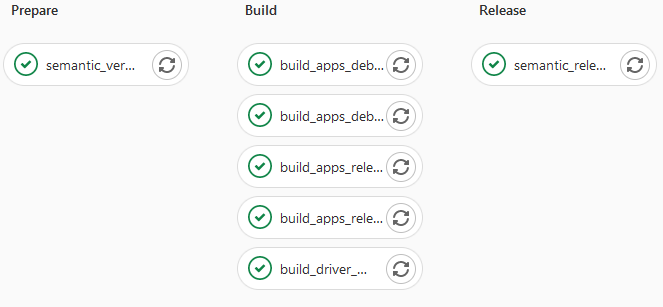
\includegraphics[width=\textwidth]{semantic_release_pipeline}
    \caption{Etapy procesu automatyzacji z wykorzystaniem \emph{semantic-release}.}
    \label{fig:semantic_pipeline}
\end{figure}

Zasady dokonywanej przez \emph{semantic-release} analizy wiadomości, istniejącej w ramach rewizji, zostały ustandaryzowane według konwencji \emph{ESLint} \cite{eslint}. W przypadku, gdy powinno zostać utworzone nowe wydanie, należy wraz z nową rewizją przygotować wiadomość w następującym formacie: \lstinline{<tag>: <opis>}, gdzie \lstinline{<tag>} to jedna z następujących wartości:
\begin{itemize}
    \item Fix - naprawa błędu
    \item Update - usprawnienie kompatybilne wstecz
    \item New - nowa funkcjonalność
    \item Breaking - zmiany niekompatybilne wstecz
    \item Docs - zmiany w dokumentacji
    \item Build - zmiany w procesie budowania
    \item Upgrade - zmiany w zależnościach
    \item Chore - zmiany, które w żaden sposób nie wpływają na użytkowanie, np.: zmiany w testach
\end{itemize}
Opisem może być dowolna wiadomośc krótko podsumowująca dokonane zmiany. Technologia \emph{semantic-release} ustala automatycznie na podstawie analizowanych tagów, stosując zasady \emph{semantic-versioning}, odpowiednią informację o wersji. Przykładowe działania projektu \emph{semantic-release} zostało przedstawione na listingu \ref{lst:analyze}.

\begin{lstlisting}[
    language=cmd, 
    caption={Analiza wiadomości zawartych w rewizjach z wykorzystaniem \emph{semantic-release}.}, 
    label={lst:analyze}
]
[@semantic-release/commit-analyzer] > Analyzing commit: 
                                      Breaking: This is for presentation reasons
[@semantic-release/commit-analyzer] > The release type for the commit is major
[@semantic-release/commit-analyzer] > Analysis of 29 commits complete: major release
[semantic-release] > Completed step "analyzeCommits" of plugin 
                     "@semantic-release/commit-analyzer"
[semantic-release] > The next release version is 1.0.0
\end{lstlisting}

\subsection{Podsumowanie}
Dzięki zastosowaniu wszystkich przedstawionych kroków stworzono w projekcie GGSS scentralizowany, zautomatyzowany system wersjonowania wydań aplikacji. Wszystkie czynności potrzebne do utrzymania odpowiedniej wersji odbywają się w ramach automatyzacji opartej o GitLab CI/CD oraz projekt \emph{semantic-release}. Deweloper musi jedynie wprowadzać odpowiednie oznaczenia w wiadomościach związanych z kolejnymi rewizjami, a utworzony system automatycznie zajmie się ewaluacją wszystkich trzech komponentów kolejnej wersji, zbuduje wszystkie komponenty systemu przekazując wcześniej uzyskane dane oraz udostępni gotowe do działania aplikacje w ramach nowego wydania dostępnego na portalu GitLab.
